\section{Congestión}
\subsubsection*{Resource allocation} Es el proceso por el cual los elementos de la red tratan de satisfacer las demandas competitivas que las aplicaciones tienen para los recursos de la red, principalmente el ancho de banda del enlace y el espacio de buffer en los routers o switches.

\subsubsection*{control de congestión} 
Utilizamos el término control de congestión para describir los esfuerzos realizados por los nodos de la red para prevenir o responder a las condiciones de sobrecarga. Dado que la congestión es generalmente mala para todos, el primer orden de negocios es hacer que la congestión disminuya, o prevenirla en primer lugar. Esto podría lograrse simplemente persuadiendo a algunos hosts a dejar de enviar, mejorando así la situación para todos los demás. Sin embargo, es más común que los mecanismos de control de congestión tengan algún aspecto de equidad, es decir, tratan de compartir el dolor entre todos los usuarios, en lugar de causar un gran dolor a unos pocos. 

\subsubsection*{Flujo} 
Para esta sección vamos a asumir que la red es esencialmente sin conexión, con cualquier servicio orientado a la conexión implementado en el protocolo de transporte que se ejecuta en los hosts finales. Sin embargo, generalmente ocurre que una secuencia de datagramas entre un par de hosts particulares \textbf{fluye} a través de un conjunto particular de enrutadores,  La suposición de que todos los datagramas son completamente independientes en una red sin conexión es demasiado fuerte. Los datagramas ciertamente se conmutan independientemente, pero generalmente ocurre que una secuencia de datagramas entre un par de hosts particulares fluye a través de un conjunto particular de enrutadores. Esta idea de un flujo, una secuencia de paquetes enviados entre un par \(\langle origen , destino\rangle\) y siguiendo la misma ruta a través de la red, es una abstracción importante en el contexto de la asignación de recursos.

\subsubsection*{Soft state}
Dado que varios paquetes relacionados fluyen a través de cada enrutador, a veces tiene sentido mantener información de estado para cada flujo, información que se puede utilizar para tomar decisiones de asignación de recursos sobre los paquetes que pertenecen al mismo. Este estado a veces se llama \textbf{soft state}. Este estado representa un punto intermedio entre una red puramente sin conexión que no mantiene ningún estado en los enrutadores y una red puramente orientada a la conexión que mantiene un \textbf{hard state} en los enrutadores. En general, el funcionamiento correcto de la red no depende de que el \textbf{soft state} esté presente (cada paquete aún se enruta correctamente sin tener en cuenta este estado).

Un flujo puede definirse implícitamente o establecerse explícitamente. En el primer caso, cada enrutador observa los paquetes que viajan entre el mismo par de \(\langle origen , destino\rangle\) inspeccionando las direcciones en el encabezado y trata estos paquetes como pertenecientes al mismo flujo. En el último caso, la fuente envía un mensaje de configuración de flujo a través de la red, declarando que un flujo de paquetes está a punto de comenzar.

\subsubsection*{Quality of Service (QoS)} 
Con \textbf{best effort serivce}, todos los paquetes reciben el mismo tratamiento, sin que los hosts finales tengan la oportunidad de pedir a la red que algunos paquetes o flujos reciban ciertas garantías o un servicio preferencial. Hay modelos de servicios que proporciona múltiples calidades de servicio (QoS). 

\subsection{Asiganción de recursos}
\subsubsection{Caracteristicas de mecanismos de asignación de recursos}
\subsubsection*{Router Centric vs Host Centric}
Los mecanismos de asignación de recursos se pueden clasificar en dos grupos amplios: aquellos que abordan el problema desde dentro de la red y aquellos que lo abordan desde los bordes: 

En un diseño centrado en el enrutador, cada enrutador se hace responsable de decidir cuándo se reenvían los paquetes y seleccionar qué paquetes se deben descartar, así como de informar a los hosts que generan el tráfico de red cuántos paquetes se les permite enviar. En un diseño centrado en el host, los hosts finales observan las condiciones de la red y ajustan su comportamiento en consecuencia. Estos dos grupos no son mutuamente excluyentes, dado que es el caso de que tanto los enrutadores dentro de la red como los hosts en los bordes de la red participan en la asignación de recursos, el problema real es dónde recae la mayor parte de la carga.

\subsubsection*{Reserva vs Feedback}
Los mecanimos de resource allocation según si usan reservas o feedback.

En un sistema basado en reservas, alguna entidad le pide a la red una cierta cantidad de capacidad para asignar a un flujo. Cada router asigna entonces suficientes recursos (buffers y / o porcentaje del ancho de banda al enlace) para satisfacer esta solicitud. Si hay un router que no puede satisfacer el pedio porque eso comprometería sus recursos, entonces rechaza la reserva. En un enfoque basado en feedback, los hosts finales comienzan a enviar datos sin reservar primero ninguna capacidad y luego ajustan su velocidad de envío de acuerdo con el feedback que reciben. Esta retroalimentación puede ser explícita (es decir, un enrutador congestionado envía un mensaje pidiendole que reduzca la velocidad) o implícita (es decir, ajusta su velocidad de envío de acuerdo con el comportamiento observable de la red, como pérdidas de paquetes).

\subsubsection*{Window vs Rate}
Una tercera forma de caracterizar estos mecánismos es según si son basados en ventanas o en tasas (rate). TCP es uno de los protocolos basados en ventana en los que el receptor anuncia una ventana al remitente. Esta ventana corresponde a la cantidad de espacio de búfer que tiene el receptor y limita la cantidad de datos que el remitente puede transmitir; es decir, admite el control de flujo. Este mecanismo, tambien se puede usar dentro de la red para reservar espacio de búfer. También es posible controlar el comportamiento de un remitente utilizando un rate, es decir, cuántos bits por segundo el receptor o la red pueden absorber. El control basado en rates tiene sentido para muchas aplicaciones multimedia, que tienden a generar datos a una velocidad promedio y que necesitan al menos un rendimiento mínimo para ser útiles

\subsubsection{Criterios de evaluación}
Para calcular la efectividad de un esquema de asignación de recursos, se consideran las dos métricas principales de la red: throughput y delay. Queremos la mayor cantidad de throughput y la menor cantidad de delay posible. Desafortunadamente, lograr estos dos objetivos simultneamente no es feasible. Una forma segura de que un algoritmo de resource allocation aumente el throughput es permitir que tantos paquetes como sea posible entren en la red, para impulsar la utilización de todos los enlaces hasta el 100\%. El problema con esta estrategia es que aumentar el número de paquetes en la red también aumenta la longitud de las colas en cada enrutador. Las colas más largas, a su vez, significan que los paquetes se retrasan más tiempo en la red.

Para describir esta relación, algunos diseñadores de redes han propuesto han propuesto usar el ratio de throughput a delay como una métrica para evaluar la efectividad de un esquema de asignación de recursos. Este ratio es a veces referido como el poder de la red:

\begin{equation}
  \text{Power} = \frac{\text{Throughput}}{\text{Delay}} 
\end{equation}

El objetivo es maximizar este ratio, que es una función de cuánta carga tiene la red. Buscamos un sistema estable, es decir que los paquetes continúen pasando por la red incluso cuando la red está operando bajo una carga pesada. Si un mecanismo no es estable, la red puede experimentar un colapso de congestión.

\subsubsection*{Fair Resource Allocation}
Cuando varios flujos comparten un enlace en particular, nos gustaría que cada flujo reciba una parte igual del ancho de banda. Esta definición presume que una parte justa del ancho de banda significa una parte igual del ancho de banda. Pero muchas veces, partes iguales pueden no equivaler a partes justas.

Suponiendo que justo implica igual y que todos los caminos tienen la misma longitud, se propuso una métrica que se puede usar para cuantificar la equidad de un mecanismo de control de congestión. El índice de equidad de Jain se define de la siguiente manera: Dado un conjunto de throughput de flujos \((x_1, x_2, ..., x_n)\) (medido en unidades consistentes como bits / segundo), la siguiente función asigna un índice de equidad a los flujos:
\[
  f(x_1, x_2, ..., x_n) = \frac{(\sum_{i=1}^{n} x_i)^2}{n \sum_{i=1}^{n} x_i^2}
\]

El índice de equidad siempre da como resultado un número entre 0 y 1, siendo 1 la mayor equidad.

\subsection{Politicas de cola}
Independientemente de lo simple o sofisticado que sea el mecanismo de asignación de recursos, cada enrutador debe implementar una política de encolamiento que indique cómo se almacenan en búfer los paquetes mientras esperan ser transmitidos.

\subsubsection{First In First Out (FIFO)}
El primer paquete que llega a un enrutador es el primer paquete en ser transmitido. Dado que la cantidad de espacio de búfer en cada enrutador es finita, si llega un paquete y la cola (espacio de búfer) está llena, el enrutador descarta ese paquete. Esto se hace sin tener en cuenta a qué flujo pertenece el paquete o qué tan importante es el paquete. A esto a veces se le llama \textbf{tail drop}, ya que los paquetes que llegan al final de la cola FIFO se descartan.

Una variación simple es usar encolamiento de prioridad. En esta politica se marca cada paquete con una prioridad; la marca podría llevarse, por ejemplo, en el encabezado IP. Los router implementan múltiples colas FIFO, una para cada clase de prioridad y siempre transmite paquetes desde la cola de mayor prioridad si esa cola no está vacía antes de pasar a la siguiente. Dentro de cada prioridad, los paquetes aún se administran de manera FIFO. Esta idea es una pequeña desviación del modelo de entrega de mejor esfuerzo, pero no va tan lejos como para garantizar una clase de prioridad en particular y puede generar starvation si no se implementa correctamente.

\subsubsection{Fair Queueing}
Se mantiene una cola separada por cada flujo que esté pasando por el router. El router envía paquetes desde esta cola usand round-robin. Cuando un flujo manda paquetes demasiado rápido, Cuando un flujo envía paquetes demasiado rápido, entonces su cola se llena. Cuando una cola alcanza su máxima longitud, los paquetes adicionales que pertenecen a ese flujo se descartan. De esta manera, una fuente determinada no puede aumentar arbitrariamente su parte de la capacidad de la red a expensas de otros flujos.

Sin embargo, los paquetes que se procesan en un enrutador no son necesariamente de la misma longitud. Para asignar verdaderamente el ancho de banda al enlace de salida de manera justa, es necesario tener en cuenta la longitud del paquete. Por esta razon, se usa un round robint bit a bit. Fair Queueing simula este comportamiento determinando primero cuándo terminaría de transmitirse un paquete determinado si se enviara utilizando este tipo de round robin y luego utilizando este tiempo de finalización para secuenciar los paquetes para su transmisión.

Si hay \(n\) flujos activos en un router, entonces el router calcula cuanto ticks de reloj va a tardar en enviar el siguiente paquete de cada flujo y le asigna un timestamp. Al momento de transmitir, el router elige el paquete con menor timestamp.

El enlace nunca queda inactivo si hay al menos un paquete en la cola. Cualquier esquema de encolamiento con esta característica se dice que conserva el trabajo. Si el enlace está completamente cargado y hay \(n\) flujos enviando datos, no puedo usar más de \(1/n\) th del ancho de banda del enlace. Si intento enviar más que eso, mis paquetes se asignarán cada vez más grandes marcas de tiempo, lo que hará que se sienten en la cola más tiempo esperando la transmisión.

Es posible implementar una variación de FQ, llamada weighted fair queuing (WFQ), que permite asignar un peso a cada flujo (cola). Este peso especifica lógicamente cuántos bits transmitir cada vez que el enrutador atiende esa cola, lo que controla efectivamente el porcentaje del ancho de banda del enlace que ese flujo obtendrá.

\subsection{Control de congestión en TCP}
TCP asume que solo hay encolamiento FIFO en los routers de la red, pero también funciona con encolamiento justo.

Los hosts que desean enviar información pueden determinar cuanta capacidad de la red pueden usar usando TCP. Esto les sirve para saber cuantos paquetes pueden tener en tránsito. Una vez que transmitió esta cantidad de paquetes, usa la llegada de un ACK como una señal de que uno de sus paquetes salió de la red y que es seguro insertar uno nuevo sin agregar al nivel de congestión. Se dice que TCP es auto-regulado.

TCP mantiene una nueva variable de estado para cada conexión, llamada \textbf{CongestionWindow}, que es usada por la fuente para limitar cuanta información puede tener en tránsito en un momento dado. Se modifica el protocolo de tal manera que el número máximo de bytes de datos no reconocidos permitidos es ahora el mínimo de la ventana de congestión y la ventana anunciada.

\[\texttt{MaxWindow}= \min ( \texttt{CongestionWindow} , \texttt{AdvertisedWindow})\]

El host emisor establece la ventana de congestión en función del nivel de congestión que percibe que existe en la red. Esto implica disminuir la ventana de congestión cuando el nivel de congestión aumenta y aumentarla cuando el nivel de congestión disminuye. En conjunto, para esto utiliza un politica de aumento aditivo / disminución multiplicativa (\textbf{Additive Increase / Multiplicative Decrease} - AIMD); Cada vez que recibe un timeout, disminuye la ventana de congestión a la mitad y cada vez que recibe tantos ACK como paquetes haya enviado, aumenta la ventana de congestión en 1 MSS (Maximum Segment Size).

Este patrón de aumentar y disminuir continuamente la ventana de congestión continúa durante toda la vida útil de la conexión. De hecho, si traza el valor actual de CongestionWindow como una función del tiempo, obtiene un patrón de dientes de sierra.

\begin{figure}[H]
	\centering
	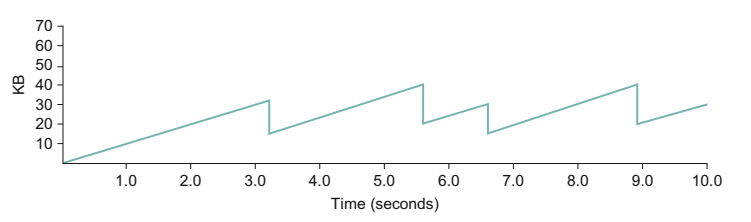
\includegraphics[width=0.7\textwidth
]{images/tcp-congestion.png}
	\caption[TCP Window Size]{TCP Window Size}
	\label{fig:tcp-congesiton}
\end{figure}

\subsubsection{Slow Start}
El mecanimos recién descripto se utiliza cuando el source host ya está haciendo uso de casi toda la capacidad disponible de la red. Cuando la conexión recién comienza, TCP setea la ventada de congestión en 1 MSS. Cada vez que recibe un ACK, aumenta la ventana de congestión en 1 MSS y transmite 2 paquetes. Cuando recibe todos los correspondientes a los paquetes en transmisión en ese momento, duplica la ventana de congestión. De esta forma, este valor aumenta exponencialmente hasta que se llega a perder el primer paquete. Aquí es donde se comienza a usa AIMD.

Slow start también se vuelve a usar en el caso de que la conexión haya quedado idle por un tiempo. Es decir, si la ventana de transmisión se redujo a cero.

\subsubsection*{Retransmisión y recuperación rápidas}
Cada vez que un paquete de datos llega al lado receptor, el receptor responde con un ACK, incluso si este número de secuencia ya ha sido reconocido. 

Cuando llega un paquete fuera de orden, TCP no puede reconocer los datos que contiene porque los datos anteriores aún no han llegado, entonces reenvía el mismo Ack que envió la última vez. Esta segunda transmisión se llama ACK duplicado. Cuando el lado emisor ve un ACK duplicado, sabe que el otro lado debe haber recibido un paquete fuera de orden, lo que sugiere que un paquete anterior podría haberse perdido. Dado que también es posible que el paquete anterior solo se haya retrasado en lugar de perdido, el remitente espera hasta que ve algunos ACK duplicados y luego retransmite el paquete faltante. En la práctica, TCP espera hasta que ha visto tres ACK duplicados antes de retransmitir el paquete.

En general, esta técnica puede eliminar aproximadamente la mitad de los tiempos de espera en una conexión TCP típica, lo que resulta en una mejora de aproximadamente el 20\% en el rendimiento sobre lo que de otro modo se podría haber logrado. 

Cuando el mecanismo de retransmisión rápida detecta la congestión, en lugar de reducir la ventana de congestión a un paquete y ejecutar el slow start, es posible utilizar los ACK que todavía están en transmición para sincronizar el envío de paquetes. Este mecanismo, que se llama recuperación rápida, elimina efectivamente la fase de inicio lento que ocurre entre cuando la retransmisión rápida detecta un paquete perdido y el aumento aditivo comienza.

\subsubsection{Congestion Avoidance}
TCP necesita crear pérdidas para encontrar el ancho de banda disponible de la conexión. Una alternativa atractiva, pero que aún no se ha adoptado ampliamente, es predecir cuándo está a punto de ocurrir la congestión y luego reducir la velocidad a la que los hosts envían datos justo antes de que comiencen a descartarse los paquetes.

\subsubsection*{DECbit}
Cada enrutador monitorea la carga que está experimentando y notifica explícitamente a los nodos finales cuando está a punto de ocurrir una congestión. Esta notificación se implementa estableciendo un bit de congestión binario en los paquetes que fluyen a través del router. El host de destino copia este bit de congestión en el ACK que envía de vuelta a la fuente.

La fuente registra cuántos de sus paquetes resultaron en que algún enrutador estableciera el bit de congestión. En particular, la fuente mantiene una ventana de congestión, al igual que en TCP, y observa qué fracción de la última ventana de paquetes resultó en que se estableciera el bit. Si menos del 50\% de los paquetes de la ventana resultaron en que se estableciera el bit, la fuente aumenta su ventana de congestión en 1 MSS. Si más del 50\% de los paquetes de la ventana resultaron en que se estableciera el bit o hubo un timeout, la fuente reduce su ventana de congestión a la mitad.

\subsubsection*{Random Early Detection (RED)}
Cada router está programado para monitorear su propia longitud de cola y, cuando detecta que la congestión es inminente, notificar (de manera implicita) a la fuente para que ajuste su ventana de congestión.

Esta notificación se implementa descartando paquetes antes de que la cola se llene. El router descarta paquetes de manera aleatoria, la probabilidad de descartar un paquete aumenta a medida que aumenta la longitud de la cola.

La fuente se da cuenta de esto cuando se produce el timeout para el paquete descartado o cuando recibe un ACK duplicado. En cuyo caso, reduce su ventana de congestión.

Para calcular la probabilidad con la que debe descartar un paquete, cada router calcula la longitud promedio ponderada de la cola:
\[
    \texttt{AvgLen} = (1 - \texttt{Weight}) \times \texttt{AvgLen} + \texttt{Weight} \times \texttt{SampleLen}
\]

donde \(0\leq \texttt{Weight} \leq 1\) y \(\texttt{SampleLen}\) es la longitud de la cola en el momento en que se realiza la medición. En la mayoría de los casos ,este momento es cuando se recibe un paquete.

El promedio ponderado trata de detectar congestiones de larga duración. En el caso de que la cola del router se llene y vacie rapidamente sería erroneo notificar una congestión (esta situación es muy normal en el internet, dada la naturaleza de la transición que se realiza en ráfagas y no de manera uniforme a través del tiempo)

El router tiene configurado dos cotas para la longitud de la cola: \texttt{MinThreshold} y \texttt{MaxThreshold}  Si \(\texttt{AvgLen} < \texttt{MihThreshold}\) entonces no se descarta ningún paquete. Si \(\texttt{AvgLen} > \texttt{MaxThreshold}\) entonces se descarta cada paquete. Si \(\texttt{MinThreshold} < \texttt{AvgLen} < \texttt{MaxThreshold}\) entonces se descarta cada paquete con probabilidad \(P\) donde:

\[
    \texttt{TempP} = \texttt{MaxP}\times\frac{\texttt{AvgLen} - \texttt{MinThreshold}}{\texttt{MaxThreshold} - \texttt{MinThreshold}}
\]

\[
  P = \frac{\texttt{TempP}}{1 - \texttt{count}\times\texttt{TempP}}
\]

con \texttt{count} la cantidad de paquetes se encolaron y \(\texttt{MaxP} = 0.02\).

La naturaleza aleatoria de RED confiere una propiedad interesante al algoritmo. La probabilidad de que se decida descartar los paquetes de un flujo en particular es aproximadamente proporcional a la parte del ancho de banda que ese flujo está recibiendo actualmente en ese router. Esto se debe a que un flujo que envía una cantidad relativamente grande de paquetes proporciona más candidatos para descartar al azar. Por lo tanto, hay cierto sentido de asignación justa de recursos incorporado en RED, aunque de ninguna manera es preciso.
